\chapter{My Tribute to Professor G. Ramachandran}\label{chap32}

\Authorline{Yee Yee Oo}

\authinfo{Pro-rector, Taungoo University Myanmar}

Hello. I am Yee Yee Oo from Myanmar. As soon as I heard about the commemorative volume of articles as a tribute to our respected teacher, Professor G. Ramachandran, who passed away on 9$^{\rm th}$ April, 2020, the foremost thoughts that came to my mind was to express and speak out my deep gratitude towards him. I always recall his kindness and great support to me when I was doing my Ph.D. in Bangalore University. That is why, I wish to recall and share some unforgettable memories of my association with him.  

I received an Indian Government Scholarship, under the India Council of Cultural Relation Program in 2000. I joined Physics Department, Bangalore University, under the joint guidance of Prof.\ Sharath Ananthamurthy, from Department of Physics, Bangalore University, and Prof.\ K. N. Nagendra from Indian Institute of Astrophysics (IIA), to carry out research towards Doctoral Degree. So, I often visited IIA to meet my supervisor KNN sir and work there. 

One day, during my study in IIA, a memorable event occurred! KNN sir took me to one of the Professor's offices where I met Professor G. Ramachandran. I was introduced to Professor GR by KNN sir and came to know that Professor GR had joined IIA as an Emeritus Scientist. Professor GR sir asked me to give a talk about my doctoral work. 

Then, I presented my research work to Professor GR sir and KNN sir and all other research candidates and tried to answer his questions. I could not answer well and finally I cried in front of the audience. He smiled and said that he understood a girl's feelings because he was also the father of daughters. He encouraged me not to worry and he promised to help me complete my doctoral work.  I could not forget about his empathy as well as ``metta" (loving kindness) and it made me feel good. Everyone, who is away from home, can understand my feelings. Since that day, I became one of the students of Professor GR sir. Later, I often visited Professor GR sir at his home and worked for my research as well as prepared the research papers for publication. Whenever I left his home late in the evening, he would tell me ``Ms. Oo, give me a ring when you reach your place"! How lovely he was!! We can see his kindness and care towards his students. Such kind of metta made me stay in Bangalore happily for five years and complete my Ph.D. degree successfully! Deep empathy, kindness, and care shown towards me by all my teachers, including Professor GR sir, provided me the strength to overcome homesickness, loneliness and motivation to carry on with my studies. 

A memorable event occurred again recently. Last November 2019, I got a chance to attend the International Programme in Educational Management for Myanmar Educational Administrators at National Institute of Educational Planning and Administration (NIEPA), New Delhi, supported by Indian Technical and Economic Cooperation (ITEC). On that occasion, I got a chance to speak with Professor GR sir and he asked me to visit Bangalore. He said he will arrange a Talk by me about my progress, as a Ph.D. holder and as one of his students. However, I had a very tight schedule and I could not visit him. Even though I have mentioned just two events above, I always remember that he usually kept in touch me and wanted me to let him know all my circumstances through many emails. Also, he, as a good teacher, was always interested in my progress and development. 

I received the sad message from Professor Sharath sir that ``Professor GR sir passed away on 9$^{\rm th}$ April 2020". I was deeply shocked to hear about the loss of my dearest teacher. Before that sad news, I also received the sad news of KNN sir who passed away on 6$^{\rm th}$ March 2020 from Professor Sharath sir. I have lost my two great supervisors within a short period. I lost a chance to meet them again since my return to Myanmar from India in 2005. My great desire is to visit Bangalore again and pay my respects to all my supervisors when we all are alive. So, I am thinking and planning to visit Bangalore during Winter of 2020 to express a great debt of gratitude to all my teachers. I deeply regret that I could not visit Bangalore last November 2019. 

I can never express enough gratitude for the help and guidance I received from Professors GR sir and KNN sir by just writing this short Note. I would like to do as much as I can to cherish their memory. Therefore, I am doing a good deed by remembering them when I pray to Lord Buddha every morning. By doing so, I strongly believe that my teachers are resting in peace. 
\vspace{1cm}

\centerline{\includegraphics[scale=.8]{authorsphotos/YeeYeeOo.eps}}
\medskip

\noindent
\textbf{Dr.\ Yee Yee Oo} obtained the M.Sc.\ degree from University of Mandalay, Myanmar, in 1995, and Ph.D. from Bangalore University in 2005. She joined the Department of Physics, University of Mandalay, Myanmar, as Assistant Lecturer in 2005, and became a Professor in 2016. In 2018 she moved to Taungoo University, Myanmar, where she is currently Pro-Rector.
